\documentclass[12pt,a4paper]{article} 

\usepackage{fn2kursstyle}
\usepackage[russian]{babel}
\usepackage[T2A]{fontenc} 
\usepackage[utf8]{inputenc} 
\usepackage{geometry}
\usepackage{mathtools}
\usepackage{tikz}
\usepackage{chngcntr}

\counterwithout{equation}{section}
\counterwithout{figure}{section}
\graphicspath{{pic/}}
\frenchspacing 

\makeatletter
\newcommand*{\rom}[1]{\expandafter\@slowromancap\romannumeral #1@}
\makeatother

\title{МАТЕМАТИЧЕСКОЕ МОДЕЛИРОВАНИЕ ТЕРМОУПРУГОГО РАЗРУШЕНИЯ ХРУПКОГО МАТЕРИАЛА}
\group{ФН2-52Б}
\author{А.\,И.~Токарев}
\supervisor{М.\,П.~Галанин}
\date{2021}

\DeclareMathOperator{\Tr}{tr}

\newcommand*\circled[1]{\tikz[baseline=(char.base)]{
            \node[shape=circle,draw,inner sep=2pt] (char) {#1};}}

\makeatletter
\newenvironment{sqcases}{%
  \matrix@check\sqcases\env@sqcases
}{%
  \endarray\right.%
}
\def\env@sqcases{%
  \let\@ifnextchar\new@ifnextchar
  \left\lbrack
  \def\arraystretch{1.2}%
  \array{@{}l@{\quad}l@{}}%
}
\makeatother

\makeatletter
\newcommand{\oset}[3][0ex]{%
  \mathrel{\mathop{#3}\limits^{
    \vbox to#1{\kern-2\ex@
    \hbox{$\scriptstyle#2$}\vss}}}}
\makeatother

\begin{document}
    \maketitle
    \tableofcontents
    \pagebreak

    \section-{Введение}
    

    \section{Постановка задачи}

    В трехмерном пространстве тензор второго ранга проще всего представить как матрицу, заданную в каждой точке пространства и описывающую неоднородность (в твердых телах -- шереховатости, потертости, микротрещины) этого пространства. Тензор, действуя на входящий вектор, изменяет его направление и масштаб. В общем случае напряжения и деформации также описываются тензорами второго ранга. 

    \subsection{Тензор малых деформаций Коши}

    Под действием внешних сил в твердом теле возникают деформации, иными словам -- изменение его формы и объема. Если разбить тело на систему точек $X_i(x_1 \ldots x_n)$, а также задать радиус-вектор $\vec r_i$ = $\vec r(X_i)$ = $\vec r(x_1 \ldots x_n)$ для каждой из них, причем
    \[
        r_i = \Bigl[ \, \displaystyle \sum_{k = 1}^{n} (x_j - 0)^2 \, \Bigr]^\frac{1}{2} = \Bigl[ \, \displaystyle \sum_{k = 1}^{n} x_j^2 \, \Bigr]^\frac{1}{2},
    \]

    \noindent то деформацию $\vec u$ (вектор деформации, вектор смещения)$[1]$ тела в каждой точке можно определить, как разницу между положением до и после приложения силы:
    \begin{equation}
      \vec u(u_1 \ldots u_n) = \vec r(X_i^') - \vec r(X_i) = \vec r^{\, '} - \vec r
      \label{shift}
    \end{equation}

    Рассмотрим две соседние бесконечно близкие точки, тогда разность расстояния между ними до начала процесса деформации задается величиной $dX$, а после -- $dX^'$. Воспользовавшись определением вектора деформации (\refeq{shift}) получим
    \[
      dX^' = dX + du \Rightarrow dx_k^' = dx_k + du_k
    \]

    \noindent а расстояния $dl$ и $dl^'$ между заданными точками до и после деформации соответственно вычисляются по определению: 
    \[
        \begin{split}
          dl &= \Bigl[ \, \displaystyle \sum_{k = 1}^{n} (dx_k)^2 \, \Bigr]^\frac{1}{2} \\
          dl^' &= \Bigl[ \, \displaystyle \sum_{k = 1}^{n} (dx_k^')^2 \, \Bigr]^\frac{1}{2} = \Bigl[ \, \displaystyle \sum_{k = 1}^{n} (dx_k + du_k)^2 \, \Bigr]^\frac{1}{2}
        \end{split}
    \]

    По определению полного дифференциала $du_k = \displaystyle \sum_{l = 1}^{n} \dfrac{\partial u_k}{\partial x_l} dx_l$. Дадим конкретный физический смысл полученной величине.  

    Пусть $ x_1 = x,\, x_2 = y,\, x_3 = z $, а координаты вектора смещения зададим, как $ u = u(u_1, u_2, u_3)$, тогда 
    \[
      \begin{split}
        du_1 &= \dfrac{\partial u_1}{\partial x}dx + \dfrac{\partial u_1}{\partial y}dy + \dfrac{\partial u_1}{\partial z}dz = \Delta_{11}dx + \Delta_{12}dy + \Delta_{13}dz  \\[0.7em]
        du_2 &= \dfrac{\partial u_2}{\partial x}dx + \dfrac{\partial u_2}{\partial y}dy + \dfrac{\partial u_2}{\partial z}dz = \Delta_{21}dx + \Delta_{22}dy + \Delta_{23}dz\\[0.7em]
        du_3 &= \dfrac{\partial u_3}{\partial x}dx + \dfrac{\partial u_3}{\partial y}dy + \dfrac{\partial u_3}{\partial z}dz = \Delta_{31}dx + \Delta_{32}dy + \Delta_{33}dz \\
      \end{split}
    \]

    Пусть деформация происходит только в направлении $x$, значит $dy = dz = 0$ и тогда 
    \[
      \begin{split}
        du_1 &= \dfrac{\partial u_1}{\partial x}dx = \Delta_{11}dx \\[0.7em]
        du_2 &= \dfrac{\partial u_2}{\partial x}dx = \Delta_{21}dx \\[0.7em]
        du_3 &= \dfrac{\partial u_3}{\partial x}dx = \Delta_{31}dx
      \end{split}
    \]
    
    Величина $ \Delta_{11} $ -- это растяжение (сжатие) отрезка $dx$, спроецированного на ось $x$. Аналогичным образом определяются $\Delta_{22}, \Delta_{33}$ растяжения (сжатия) вдоль осей \nolinebreak{$y, z$}

    Компоненты $\Delta_{21},\, \Delta_{31}$ определяют поворот параллельно оси $x$: в первом случае -- вокруг оси $z$ в сторону $y$ (против часовой стрелки), а во втором -- вокруг оси $y$ в сторону оси $z$ (против часовой стрелки). 
    
    Если деформация происходит по всем направлениям, то $\Delta_{12}$ определяет поворот параллельно оси $y$ вокруг оси $z$ в направлении $x$ (по часовой стрелке), а $ \Delta_{13} $ -- вокруг оси $y$ в направлении оси $x$ (по часовой стрелке). Компоненты $\Delta_{23}, \Delta_{32}$ определяют повороты вокруг оси $x$: в первом случае -- в направлении оси $y$ (по часовой стрелке), во втором -- в направлении $z$ (против часовой стрелки). Пример деформации приведен на рис. \ref{fig:deform}

    \begin{figure}[h]
      \centering
      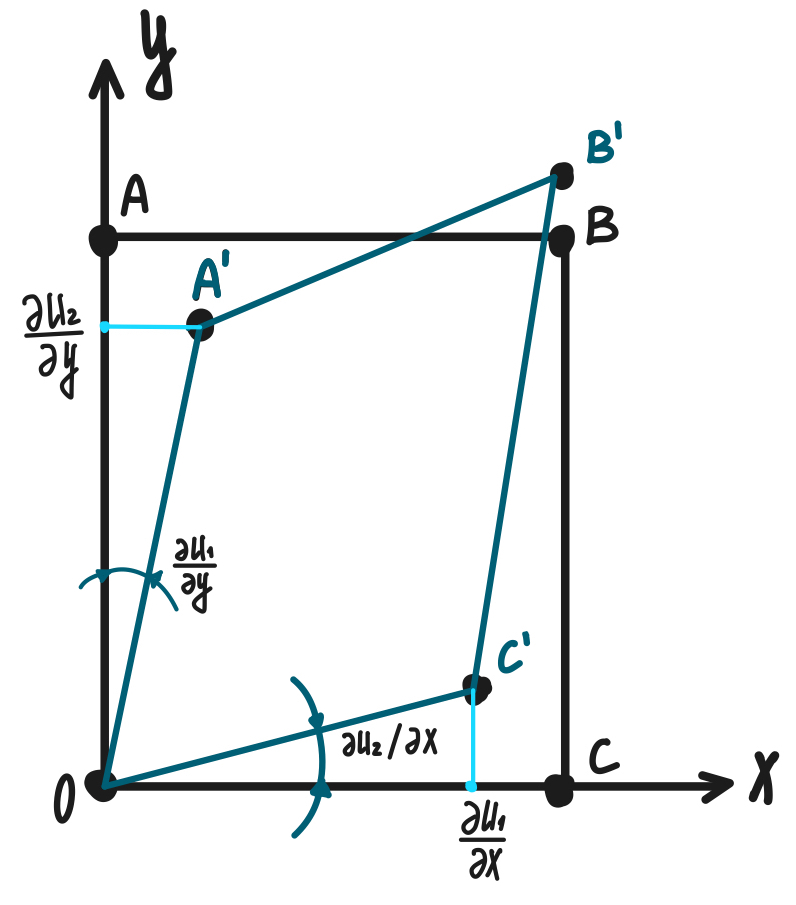
\includegraphics[width=0.5\textwidth]{deform.jpeg}
      \caption{Процесс деформации}
      \label{fig:deform}
    \end{figure}
    
    Используя все проделанные раннее рассуждения, преобразуем элемент расстояния $(dl^')^2$ к виду:
    \[
      \begin{split}
        (dl^')^2 &= (dl)^2 + 2 \displaystyle \sum_{k = 1}^{n} dx_k du_k + \displaystyle \sum_{j = 1}^{n} (du_k)^2 = (dl_i)^2 + 2 \displaystyle \sum_{k = 1}^{n} \displaystyle \sum_{l = 1}^{n} \dfrac{\partial u_k}{\partial x_l} dx_l dx_k \, + \\
        &+ \displaystyle \sum_{k = 1}^{n} \displaystyle \sum_{l = 1}^{n} \Bigl(\dfrac{\partial u_k}{\partial x_l} dx_l \Bigr)^2
      \end{split}
    \]

    Запишем в более лаконичном виде:
    \begin{equation}
      \begin{split}
        (dl^')^2 &= (dl)^2 + 2 \dfrac{\partial u_k}{\partial x_l} dx_l dx_k + \Bigl(\dfrac{\partial u_k}{\partial x_l} dx_l \Bigr)^2
      \end{split}
    \end{equation}

    При малых деформациях третьим слагаемым можно пренебречь в силу его большего порядка малости. 

    Во втором слагаемом индексы $j, k$ являются немыми, поэтому его можно записать в симметричном виде
    \begin{equation}
      \dfrac{\partial u_k}{\partial x_l} dx_l dx_k = \dfrac{1}{2} \Bigl( \dfrac{\partial u_k}{\partial x_l} + \dfrac{\partial u_l}{\partial x_k} \Bigr)dx_l dx_k = \varepsilon_{kl} dx_l dx_k,
      \label{deformTensorComponent}
    \end{equation}
    \noindent где $\varepsilon_{kl}$ -- составляющая тензора деформаций в точке $X$. 
    
    В предположении существования аддитивного разложения компонент тензора деформаций Коши запишем:
    \[
      \varepsilon_{kl} = \dfrac{1}{2}\Bigl( \dfrac{\partial u_k}{\partial x_l} + \dfrac{\partial u_l}{\partial x_k} \Bigr) = \varepsilon_{kl}^e +  \varepsilon_{kl}^0, \quad k, l = 1, 2, 3,
    \]
    \noindent где $\varepsilon_{kl}^e$ -- компоненты упругой состовляющей тензора деформаций, а $ \varepsilon_{kl}^0 $ -- компоненты тенхора неупругих деформаций среду (в нашем случае температурные деформации).
    
    Термоупругость описывает деформации при неравномерном нагреве деформируемых тел. Термоупругое тело обладает хотя бы одним естественным состоянием, в котором отсутствуют напряжения и деформации, при том температура во всех точках одинакова. Свяжем это состояние с начальной температурой тела $T_0$. При нагреве или охлаждении в теле возникают температурные деформации, описываемые тензором с компонентами $ \varepsilon_{kl}^0 \colon$
    \[
      \varepsilon_{kl}^0 = \alpha_{kl}^T \Delta T \Rightarrow \varepsilon_{kl}^0 \sim \alpha_{kl}^T,
    \]
    \noindent где $ \alpha_{kl}^T $ -- компоненты тензора теплового расширения.

    \subsection{Тензор напряжений}

    Напряжением будем называть меру внутренних сил, возникших в результате приложения внешней силы. 

    Рассмотри элементарный объем тела -- куб (рис. \refeq{fig:cube}). Если само тело находится в статическом равновесии, то силы, действующие на параллельные грани куба равны по модули, но разные по направлению. Поэтому можно рассмотреть только те силы, которые действуют на непараллельные грани куба.

    \pagebreak

    \begin{figure}[h]
      \centering
      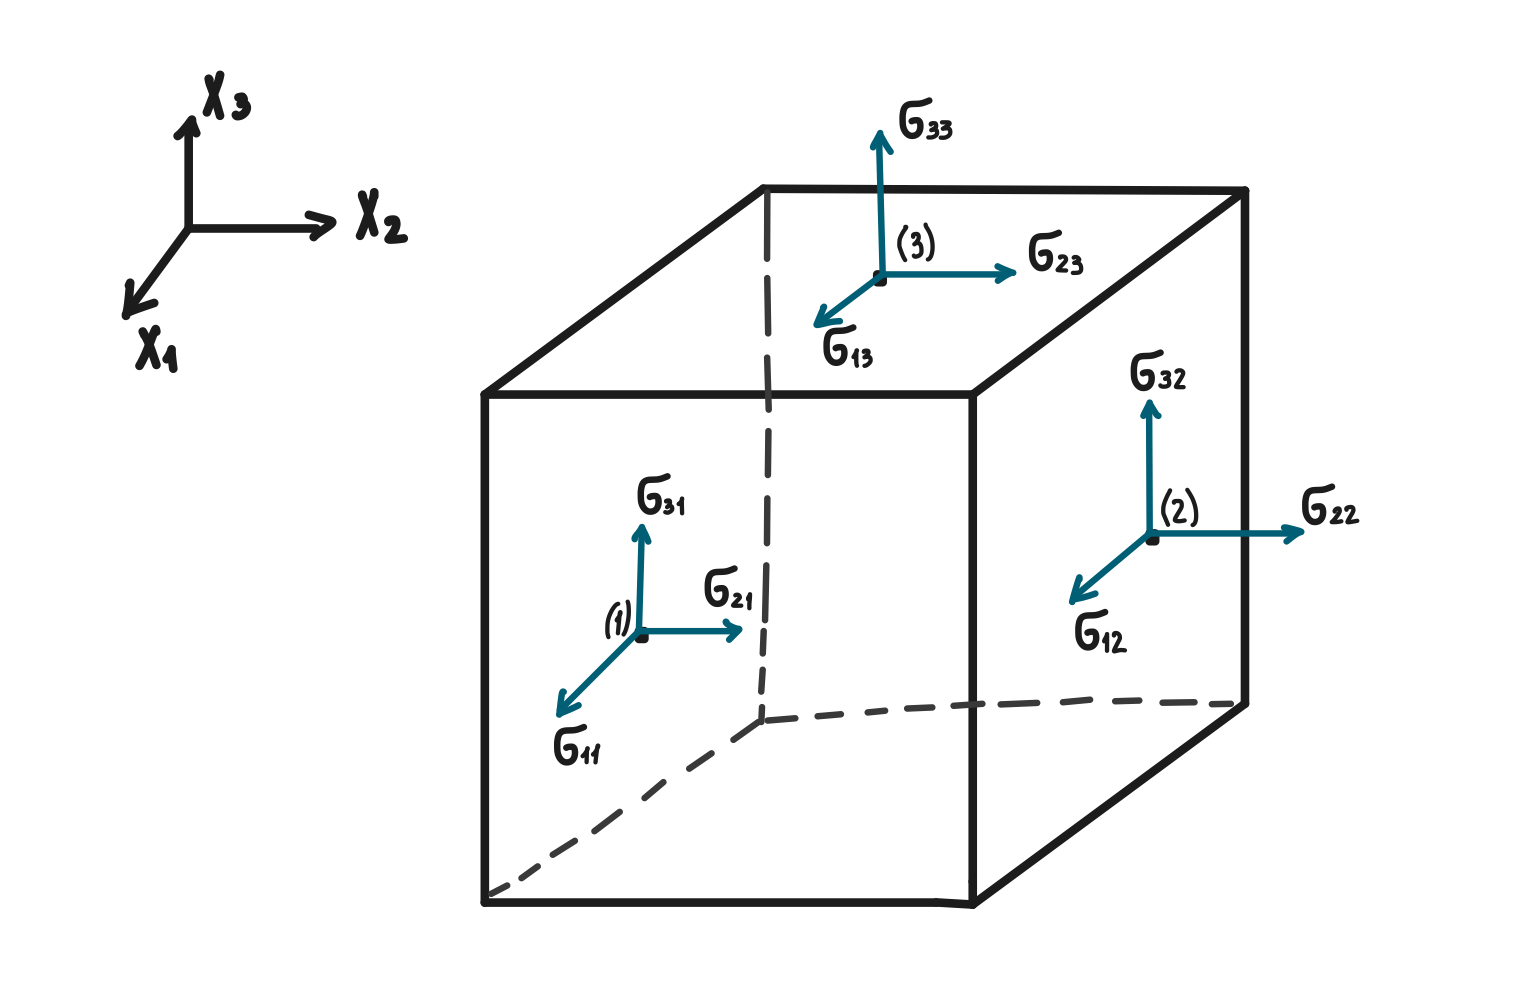
\includegraphics[width=0.65\textwidth]{cube.jpeg}
      \caption{Проекции напряжений в элементарном объеме тела}
      \label{fig:cube}
    \end{figure}

    \begin{figure}[h]
      \centering
      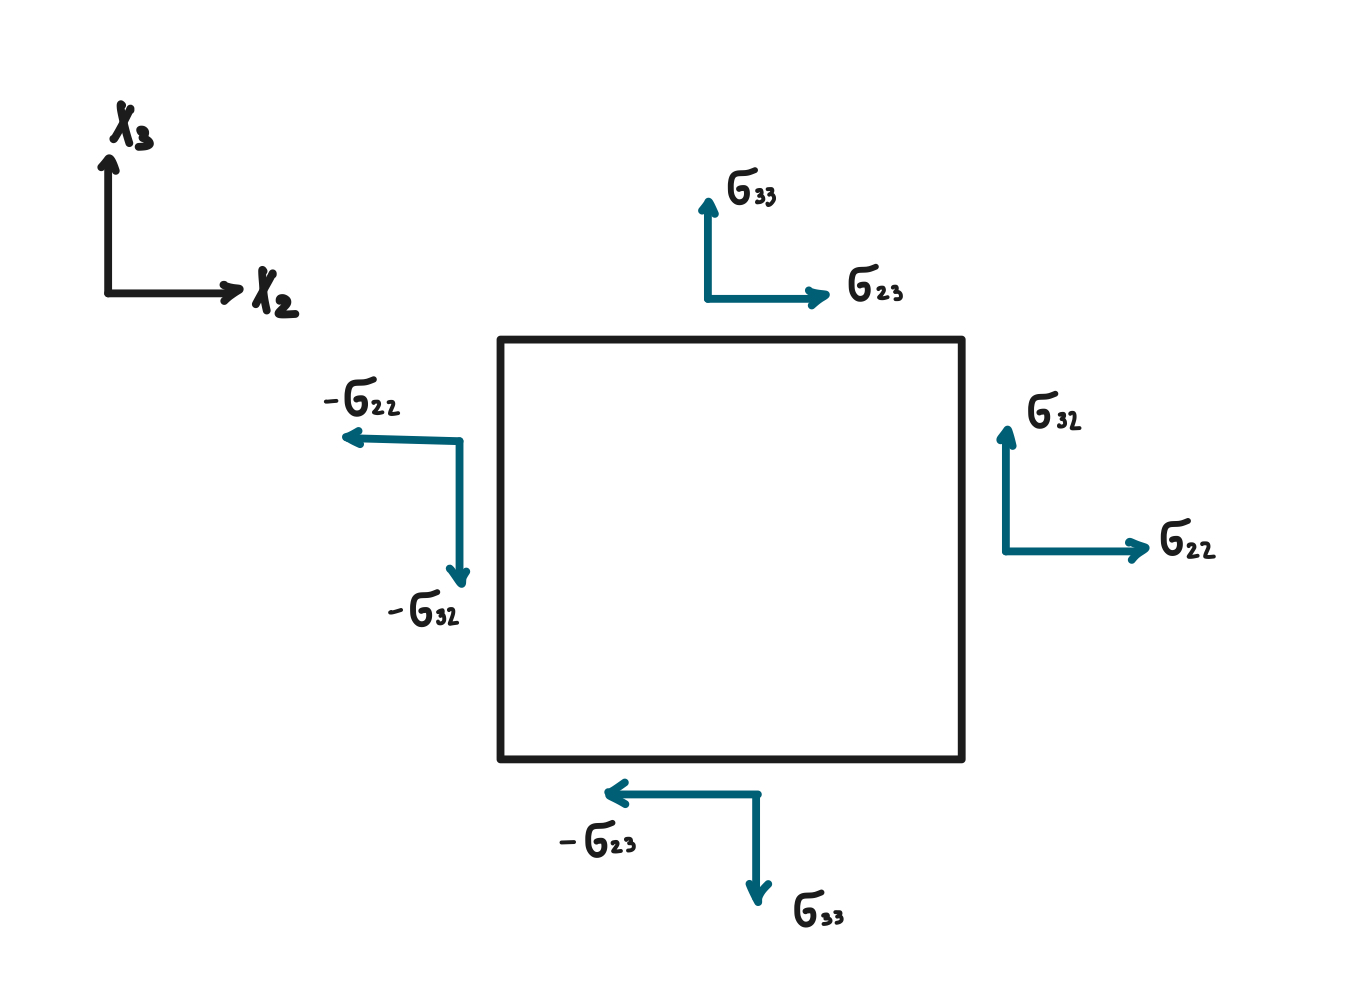
\includegraphics[width=0.65\textwidth]{cube_cut.jpeg}
      \caption{Проекции напряжений на ось $x_1x_2$, проходящую через центр куба}
      \label{fig:cube_cut}
    \end{figure}

    \pagebreak

    Выделим какую-нибудь из плоскостей, вырезанную из тела (рис. \refeq{fig:cube_cut}). Равнодействующая всех сил, а также сумма всех моментов равны нулю (следует из статического равновесия). Этот факт позволяет нам сделать вывод о том, что $\sigma_{23} = \sigma_{32}$, а значит в общем случае:
    \[
      \sigma_{ij} = \sigma_{ji},
    \]

    \noindent то есть тензор напряжений симметричен.

    \subsection{Поведение свойств среды (анизотропия, ортотропия и изотропия)}

    Анизотропия -- это различие свойств среды (в нашем случае упругости и теплопроводности) в зависимости от направления. Примерами анизотропных тел являются разлиыне кристаллы. Если вырезать две части (одну вдоль оригинального образца, а другую -- поперек), то они покажут разные растяжение и сжатие. 

    Ортотропия (ортогональная анизотропия) -- это симметрия свойств тела по одному из 2-3 направлений. Например, древесина очень жесткая вдоль волокон и менее жесткая в радиальном направлении от них.

    Изотропия –- это, в свою очередь, неизменность свойств среды во всех направлениях. Примерами изотропных тел являются бетон, пластик и металлы. 
    
    Характер поведения свойств тел можно определить только экспериментально.

    \subsection{Определяющее соотношение (закон Гука)}

    В реальной жизни большинство тел являются анизотропными, поэтому стандартный закон Гука уже недостаточен для описания их физических свойств. Чтобы решить эту проблему, необхоидмо ввести понятие обобщенного закона Гука, определяющего линейную зависимость между компонентами тензоров напряжений и деформаций:
    \begin{equation}
      \sigma_{ij} = C_{ijkl}\varepsilon_{ij}^e = C_{ijkl}( \varepsilon_{ij} - \varepsilon_{ij}^0 ), \quad i,j,k,l = 1, 2, 3
      \label{Hook}
    \end{equation}

    Тензор $C_{ijkl}$ упругих постоянных связывает два тензора второго ранга. Поскольку тензоры деформаций и напряжений симметричные с $6$ независимыми компонентами, то $C_{ijkl}$ будет иметь всего $6*6 = 36$ компонент. Но он еще и симметричен относительно перестановки пар индексов: 
    \[
        C_{ijkl} = C_{klij},
    \]

  \noindent поэтому имеет всего 21 независимую компоненту.

  Для последующих рассуждений нам понадобится нотация Фойгта -- матричная форма записи тензора 4 ранга (симметричный по паре индексов тензор может быть записан в виде матрицы $6{\text x}6$):
  \begin{equation}
    \begin{split}
        11 &\rightarrow 1 \\
        22 &\rightarrow 2 \\
        33 &\rightarrow 3 \\
        23,\, 32 &\rightarrow 4 \\
        13,\, 31 &\rightarrow 5 \\
        12,\, 21 &\rightarrow 6 \\
    \end{split}
    \label{Foigt}
  \end{equation}

  Выведем некоторые закономерности для кубического симметричного кристалла (ортотропное тело). 
  \begin{enumerate}
    \item В силу симметрии кристалл должен иметь одну и ту же жесткость в направлении всех осей, задающих систему координат, то есть $C_{iiii} = \linebreak = {\text const}, \, i = 1, 2, 3$. В частности, для трехмерного случая можно записать:
    \[
      C_{1111} = C_{2222} = C_{3333} \,\, \oset[2.6mm]{(\refeq{Foigt})}{\Leftrightarrow} \,\, C_{11} = C_{22} = C_{33}
    \]

    \item Вдоль пространственных диагоналей направлены оси симметрии третьего порядка (симметричность относительно поворота на $120^{\circ}$):
    \[
      \begin{split}
      C_{1212} &= C_{1313} = C_{2323} \,\, \oset[2.6mm]{(\refeq{Foigt})}{\Leftrightarrow} \,\, C_{44} = C_{55} = C_{66} \\[0.5em]
      C_{1122} &= C_{1133} = C_{2233} \,\, \oset[2.6mm]{(\refeq{Foigt})}{\Leftrightarrow} \,\, C_{12} = C_{21} = C_{13} = C_{31} = C_{23} = C_{32}
      \end{split}
    \]
    
    \item Вращательные компоненты куба не приводят к растяжению, поэтому все остальные компоненты равны нулю.
  \end{enumerate}

  \pagebreak

  Таким образом, тензору упругих постоянных можно поставить в соответствие матрицу 
  \[
    \hat{C} = 
    \begin{pmatrix}
      C_{11} & C_{12} & C_{13} & 0 & 0 & 0 \\
      C_{21} & C_{22} & C_{23} & 0 & 0 & 0 \\
      C_{31} & C_{32} & C_{33} & 0 & 0 & 0 \\
           0 &      0 &      0 & C_{44} & 0 & 0 \\
           0 &      0 &      0 & 0 & C_{55} & 0 \\
           0 &      0 &      0 & 0 & 0 & C_{66} \\
    \end{pmatrix} 
    =
    \begin{pmatrix}
      C_{11} & C_{12} & C_{12} & 0 & 0 & 0 \\
      C_{12} & C_{11} & C_{12} & 0 & 0 & 0 \\
      C_{12} & C_{12} & C_{11} & 0 & 0 & 0 \\
           0 &      0 &      0 & C_{44} & 0 & 0 \\
           0 &      0 &      0 & 0 & C_{44} & 0 \\
           0 &      0 &      0 & 0 & 0 & C_{44} \\
    \end{pmatrix} 
  \] 

  Для изотропных тел $C_{44} = C_{55} = C_{66} = \dfrac{1}{2}(C_{11} - C_{12})$. Воспользуемся параметрами Ламе:
  \[ 
    C_{11} = \lambda + 2\mu, \quad C_{12} = \lambda, \quad C_{44} = \mu,
  \]

  и подставим эти значения в матрицу $\hat{C}\colon$
  \begin{equation}
    \hat{C} = 
    \begin{pmatrix}
      \lambda + 2\mu & \lambda & \lambda & 0 & 0 & 0 \\
      \lambda & \lambda + 2\mu & \lambda & 0 & 0 & 0 \\
      \lambda & \lambda & \lambda + 2\mu & 0 & 0 & 0 \\
           0 &      0 &      0 & \mu & 0 & 0 \\
           0 &      0 &      0 & 0 & \mu & 0 \\
           0 &      0 &      0 & 0 & 0 & \mu \\
    \end{pmatrix} 
    \label{Flex}
  \end{equation}

  Возвращаясь к выражению (\refeq{Hook}) и подставив туда матрицу (\refeq{Flex}), мы получаем:
  \[
    \begin{pmatrix}
      \sigma_{11} \\
      \sigma_{22} \\
      \sigma_{33} \\
      \sigma_{23} \\
      \sigma_{13} \\
      \sigma_{12} \\
    \end{pmatrix}
    = 
    \begin{pmatrix}
      \lambda + 2\mu & \lambda & \lambda & 0 & 0 & 0 \\
      \lambda & \lambda + 2\mu & \lambda & 0 & 0 & 0 \\
      \lambda & \lambda & \lambda + 2\mu & 0 & 0 & 0 \\
           0 &      0 &      0 & \mu & 0 & 0 \\
           0 &      0 &      0 & 0 & \mu & 0 \\
           0 &      0 &      0 & 0 & 0 & \mu \\
    \end{pmatrix} 
    \begin{pmatrix}
      \varepsilon_{11} \\
      \varepsilon_{22} \\
      \varepsilon_{33} \\
      2\varepsilon_{23} \\
      2\varepsilon_{13} \\
      2\varepsilon_{12} \\
    \end{pmatrix}
  \]
  \pagebreak

  \noindent или в матричной форме

  \[
    \begin{split}
      \begin{bmatrix}
        \sigma_{11} & \sigma_{12} & \sigma_{13} \\
        \sigma_{21} & \sigma_{22} & \sigma_{23} \\
        \sigma_{31} & \sigma_{32} & \sigma_{33} \\
      \end{bmatrix}
      &= \,\,
      2\mu \begin{bmatrix}
        \varepsilon_{11} & \varepsilon_{12} & \varepsilon_{13} \\
        \varepsilon_{21} & \varepsilon_{22} & \varepsilon_{23} \\
        \varepsilon_{31} & \varepsilon_{32} & \varepsilon_{33} \\
      \end{bmatrix}
      + \lambda \begin{bmatrix}
        \varepsilon_{11} & 0 & 0 \\
        0 & \varepsilon_{22} & 0 \\ 
        0 & 0 & \varepsilon_{33} 
        \end{bmatrix}
    \end{split}
  \]

  \subsection{Уравнение равновесия}
  \begin{equation}
    \dfrac{\partial \sigma_{ji}}{x_j} + b_i = 0, \quad i = 1, 2, 3,
    \label{equillibrium}
  \end{equation}

  \noindent где $b_i$ -- это проекции вектора плотности объемных сил $b$ на оси $Ox_i$ простран- ственных координат.


  \section{Одномерный случай}


    \section-{Заключение}
    
    \newpage

    \begin{thebibliography}{9}
  

    \end{thebibliography}

    \end{document}